% !TeX root = ..//diffgeo_main.tex
\begin{bew}[Beweis Satz \ref{satz:koszulformel}]
Zu zeigen:\\
Die beiden geforderten Eigenschaften bestimmen den Zusammenhang und Koszuformel ist erfüllt.\\
Die zweite geforderte Eigenschaft impliziert:
\begin{align*}
&X g(Y, Z) = g(\covd_X Y, Z) + g(Y, \covd_X Z)\\
&Y g(X , Z) = g (\covd_Y X, Z) + g(X, \covd_Y Z)\\
&Z g(X, Y) = g(\covd_Z X, Y) + g(X, \covd_Z Y)
\end{align*}
Daraus folgt:
\begin{align*}
X g(Y, Z) + Y g(X , Z) - Z g(X, Y) &= g(\covd_X Y + \covd_Y X, Z) + g(\covd_X Z - \covd_Z X , Y)\\
 & \phantom{=}+ g(\covd_Y Z - \covd_Z Y, X) \\
 &= 2 g(\covd_X Y, Z) - g(\comm{X}{Y}, Z) + g(\comm{X}{Z}, Y) + g(\comm{Y}{Z}, X)
\end{align*}
Damit ergibt sich
\begin{align}
2 g(\covd_X Y, Z) &= g(\comm{X}{Y}, Z) - g(\comm{X}{Z}, Y) - g(\comm{Y}{Z}, X)\\
&\phantom{=} + X g(Y, Z) + Y g(X, Z) - Z g(X, Y)
\end{align}
Definiere  \ $\covd : \mathfrak{X}(\mfk) \times \mathfrak{X}(\mfk) \to \mathfrak{X}(\mfk)$
durch $\covd (X, Y)$, welches das eindeutig bestimmte glatte Vektorfeld ist, das die Koszulformel erfüllt.\\
Es bleibt zu zeigen: \
$\covd : \mathfrak{X}(\mfk) \times \mathfrak{X}(\mfk) \to \mathfrak{X}(\mfk) $ ist ein Zusammenhang.

\begin{enumerate}
\item[1) ] $\covd$ ist tensoriell im ersten Argument:
\begin{align*}
2g(\covd(\varphi X, Y),Z) &= 2g(\covd_{\varphi X}Y, Z) \\
									\phantom{.}\\
									 &= (\varphi X)(g(Y, Z)) + Y(g(\varphi X, Z)) - Z(g(\varphi X, Y)) \\
									 &\phantom{=}- g(\varphi X, [Y, Z])  - g(Y, [\varphi X, Z]) + g(Z, [\varphi X,Y]) \\
									 \phantom{.}\\
									 &= (\varphi X) g(Y, Z) + Y(\varphi)g(X, Z) +(\varphi Y)g(X, Z) \\
									 &\phantom{=}- Z(\varphi)g(X, Y) - (\varphi Z) g(X, Y) - \varphi g(X, [Y, Z]) \\
									 &\phantom{=}-\varphi g(Y, [X, Z]) + Z(\varphi) g(X, Y) - \varphi g(Z, [X, Y]) \\
									 &\phantom{=}-Y(\varphi)g(Z, X)	\\
									 \phantom{.}\\
									 &= \varphi g(\covd_XY, Z)							 
\end{align*}
\item[2) ] $\covd$ ist derivativ im zweiten Argument:
\begin{align*}
2g(\covd_X(\varphi Y), Z) &= X(g(\varphi Y, Z))	+ (\varphi Y) g(X, Z) - Z(g(X, \varphi Y))		\\
										&= g(X, [\varphi Y, Z]) - g(\varphi Y, [X, Z]) + g(Z, [X, \varphi Y]) \\
										\phantom{.}\\
										&= (\varphi X) g(Y, Z) + X(\varphi) g(Y, Z) + (\varphi Y)g(X, Z) \\
										&\phantom{=} - (\varphi Z)g(X, Y) - Z(\varphi)g(X, Y) - \varphi g(X, [Y, Z]) \\
										&\phantom{=}+ Z(\varphi)g(X, Y) - \varphi g(Y, [X, Z]) + \varphi g(Z, [X, Y]) \\
										&\phantom{=}+ X(\varphi)g(Z, Y)\\
										\phantom{.}\\
										&= 2X(\varphi) g(Y, Z) + 2\varphi g(\covd_XY,Z)																										
\end{align*}
\end{enumerate}
\end{bew}

Das nächste Ziel ist die Berechung von $\covd$ in lokalen Koordinaten. Sei also eine Karte $(x, U)$ gegeben. Mit $x_1, \dots, x_n$ bezeichnen wir den zugehörigen lokalen Rahmen. $(x_i = \frac{\partial}{\partial x_i})$
\begin{align}
\covd(x_i, x_j)= \covd_{x_i}^{\phantom{x_i}x_j} = \sum_{k=1}^{m} \Gamma^k_{ij} x_k
\end{align}
Hierbei bezeichnet man $\Gamma^k_{ij}: \mfk \longrightarrow \R$ als \textbf{Christoffel-Symbole}. \\
Sei $\covd$ nun torsionsfrei, das heißt $\covd_XY - \covd_YX = [X, Y]$.
Für $X=x_i$ und $Y=x_j$ gilt $[x_i, x_j]=0$. Damit gilt: 
\begin{align*}
\covd_{x_i}^{\phantom{x_i} x_j} - \covd_{x_j}^{\phantom{x_j}x_i} &= 0 \\
\Longleftrightarrow \quad \sum_{k=1}^{m}\Gamma^k_{ij} x_k - \sum_{k=1}^{m}\Gamma^k_{ji} x_k &= 0\\
\Longleftrightarrow \hspace{1cm} \sum_{k=1}^{m}\left[\Gamma^k_{ij} - \Gamma^k_{ji} \right] x_k &= 0
\end{align*}
Daraus erhalten wir: \ $\Gamma^k_{ij} = \Gamma^k_{ji}$ für den Fall der Torsionsfreiheit. \\
\phantom{.}\\
Sei $\nabla$ der Levi-Civita-Zusammenhang.
\begin{align*}
g(\nabla_{x_i}x_j, x_k) &= \frac{1}{2}\left[x_i(g(x_j, x_k)+ x_j(g(x_i, x_k)) - x_k(g(x_i, x_j)) \right] \\
								 &=  \frac{1}{2}(\partial_i g_{jk} + \partial_j g_{ik} - \partial_k g_{ij})
\end{align*}
\begin{align}
\nabla_{x_i}^{\phantom{x_i}x_j} = \sum_{k=1}^{m}\Gamma_{ij}^k x_k
\end{align}
\begin{align*}
g(\nabla_Xx_j, x_l) &= g\left(\sum_{k=1}^{m}\Gamma_{ij}^k x_k, x_l\right) \\
							&= \sum_{k=1}^{m}\Gamma_{ij}^k \ \underbrace{g(x_k, x_l)}_{g_{kl}}							
\end{align*}
Daraus erhalten wir eine Formel zur Berechnung der Christoffel-Symbole:
\begin{align}
\Gamma_{ij}^k = \frac{1}{2} \sum_{l}g^{kl}\left(\partial_i g_{jl} + \partial_j g_{il} - \partial_l g_{ij}\right)
\end{align}

\chapter{Geodätische}
Geodätische sind Kurven, die das Konzept der Geraden im $\R^n$ auf Mannigfaltigkeiten verallgemeinern.
Diese Verallgemeinerung ist über Zusammenhänge möglich.
\begin{figure}[H]
\centering
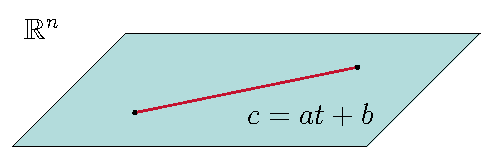
\includegraphics[width=0.6\linewidth]{figures/tikz/linern.pdf}
\caption{Gerade im $\R^n$}
\label{img:linern}
\end{figure} 
\begin{defs}[Geodätische]
Sei $\mfk$ eine Mannigfaltigkeit mit einem linearen Zusammenhang $\nabla$, $I \subseteq \R$ offen. Eine Kurve $c: I \longrightarrow \mfk$ ist eine Geodätische falls:
\begin{align} 
\label{eq:variation}
\nabla_{\frac{\partial}{\partial t}} \dot{c}(t) = 0 \qquad (\nabla_t \dot{c}(t) = 0)
\end{align}
\end{defs}
Dies ist eine Differentialgleichung, wenn wir in lokale Koordinaten übergehen.
\textbf{In lokalen Karten:} \\
Sei $(x,U)$ Karte von $\mfk$, \ $c: I \longrightarrow \mfk$ Geodätische. 
\begin{align}
c^k = x^k \circ c: \ I \longleftarrow \R
\end{align}

\begin{align}
\dot{c}(t) = \sum_k \dot{c}^k(t) \eval{\frac{\partial}{\partial x^k}}_{c(t)}
\end{align}

\begin{align*}
0=\nabla_t\dot{c}(t) &= \sum_{k=1}^{m}\nabla_t(\dot{c}^k(x_k\circ c)) \\
							   &= \sum_k \ddot{c}^k(t)(x_k\circ c) + \dot{c}^k(t)\nabla_{\dot{c}(t)}x_k \\
							   &= \sum_k \left(\ddot{c}_k(t) + \sum_{i,j}\dot{c}^{i}\dot{c}^j \Gamma_{ij}^k c(t)\right) x_k \circ c
\end{align*}

Wir betrachten die Kurve $\gamma(t)= \begin{pmatrix}
x(t) \\ y(t) \\z(t) \end{pmatrix}$. \\

Durch auswerten der zuvor hergeleiteten Gleichung erhalten wir:



